% Options for packages loaded elsewhere
\PassOptionsToPackage{unicode}{hyperref}
\PassOptionsToPackage{hyphens}{url}
%
\documentclass[
  x11names]{article}
\usepackage{amsmath,amssymb}
\usepackage{lmodern}
\usepackage{iftex}
\ifPDFTeX
  \usepackage[T1]{fontenc}
  \usepackage[utf8]{inputenc}
  \usepackage{textcomp} % provide euro and other symbols
\else % if luatex or xetex
  \usepackage{unicode-math}
  \defaultfontfeatures{Scale=MatchLowercase}
  \defaultfontfeatures[\rmfamily]{Ligatures=TeX,Scale=1}
\fi
% Use upquote if available, for straight quotes in verbatim environments
\IfFileExists{upquote.sty}{\usepackage{upquote}}{}
\IfFileExists{microtype.sty}{% use microtype if available
  \usepackage[]{microtype}
  \UseMicrotypeSet[protrusion]{basicmath} % disable protrusion for tt fonts
}{}
\makeatletter
\@ifundefined{KOMAClassName}{% if non-KOMA class
  \IfFileExists{parskip.sty}{%
    \usepackage{parskip}
  }{% else
    \setlength{\parindent}{0pt}
    \setlength{\parskip}{6pt plus 2pt minus 1pt}}
}{% if KOMA class
  \KOMAoptions{parskip=half}}
\makeatother
\usepackage{xcolor}
\usepackage[margin=1in]{geometry}
\usepackage{graphicx}
\makeatletter
\def\maxwidth{\ifdim\Gin@nat@width>\linewidth\linewidth\else\Gin@nat@width\fi}
\def\maxheight{\ifdim\Gin@nat@height>\textheight\textheight\else\Gin@nat@height\fi}
\makeatother
% Scale images if necessary, so that they will not overflow the page
% margins by default, and it is still possible to overwrite the defaults
% using explicit options in \includegraphics[width, height, ...]{}
\setkeys{Gin}{width=\maxwidth,height=\maxheight,keepaspectratio}
% Set default figure placement to htbp
\makeatletter
\def\fps@figure{htbp}
\makeatother
\setlength{\emergencystretch}{3em} % prevent overfull lines
\providecommand{\tightlist}{%
  \setlength{\itemsep}{0pt}\setlength{\parskip}{0pt}}
\setcounter{secnumdepth}{-\maxdimen} % remove section numbering
\usepackage{fontspec} \usepackage{titling} \usepackage{framed} \pretitle{\begin{center} \vspace{-3cm}
\includegraphics[width=\linewidth]{images/Base_info/logo.png}\LARGE\\} \posttitle{\end{center}} \usepackage{float} \usepackage{fancyhdr} \usepackage{ragged2e} \usepackage{caption} \usepackage{colortbl} \captionsetup[figure]{labelformat=empty} \arrayrulecolor{white} \pagestyle{fancy} \fancyhead[L,C]{} \fancypagestyle{plain}{\pagestyle{fancy}} \PassOptionsToPackage{dvipsnames,svgnames*,x11names*}{xcolor} \definecolor{ceil}{rgb}{0.57, 0.63, 0.81} \usepackage[export]{adjustbox} \usepackage{wrapfig} \usepackage{graphicx} \usepackage{caption}
\usepackage{booktabs}
\usepackage{longtable}
\usepackage{array}
\usepackage{multirow}
\usepackage{wrapfig}
\usepackage{float}
\usepackage{colortbl}
\usepackage{pdflscape}
\usepackage{tabu}
\usepackage{threeparttable}
\usepackage{threeparttablex}
\usepackage[normalem]{ulem}
\usepackage{makecell}
\usepackage{xcolor}
\ifLuaTeX
  \usepackage{selnolig}  % disable illegal ligatures
\fi
\IfFileExists{bookmark.sty}{\usepackage{bookmark}}{\usepackage{hyperref}}
\IfFileExists{xurl.sty}{\usepackage{xurl}}{} % add URL line breaks if available
\urlstyle{same} % disable monospaced font for URLs
\hypersetup{
  hidelinks,
  pdfcreator={LaTeX via pandoc}}

\author{}
\date{\vspace{-2.5em}Fecha de creación: 06 April, 2023}

\begin{document}

\renewenvironment{framed}[1][\hsize]
  {\MakeFramed{\hsize#1\advance\hsize-\width \FrameRestore}}%
  {\endMakeFramed}

\setmainfont{Arial}
\setsansfont{Arial}
\setmonofont{Arial}

\newcommand\invisiblesection[1]{%
  \refstepcounter{section}%
  \addcontentsline{toc}{section}{\protect\numberline{\thesection}#1}%
  \sectionmark{#1}}

\fancyhead[R]{\textbf{http://doi.org/10.31687/SaremLR.19.207}}

%
  \refstepcounter{section}%
  \addcontentsline{toc}{section}{\protect\numberline{\thesection}GENERALIDADES}%
  \sectionmark{GENERALIDADES}
\vspace{-0.4cm}


\includegraphics[width=1\linewidth]{images/Base_info/logo}

\vspace{1cm}

\begin{minipage}{0.7\textwidth}
\vspace{0.3cm}
\fontsize{20}{24}\selectfont\textit{Blastocerus dichotomus}

\vspace{0.3cm}
\fontsize{30}{36}\selectfont Ciervo de los pantanos
\end{minipage}
\hspace{0.05\textwidth}
\begin{minipage}{0.25\textwidth}

\includegraphics[width=\textwidth]{images/vu.png}
\end{minipage}

\normalsize

\begin{figure}[H]

{\centering 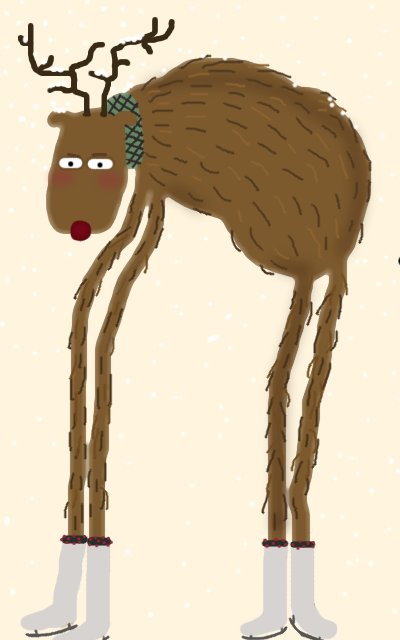
\includegraphics[width=0.35\linewidth]{photos/Blastocerus dichotomus} 

}

\caption{Fotos por Salvador Dali}\label{fig:image}
\end{figure}

\begin{center}\rule{0.5\linewidth}{0.5pt}\end{center}

\justifying

\textbf{Citar como:} Pereira, Javier A.; Varela, Diego; Aprile, Gustavo;
Cirignoli, Sebastián; Orozco, María Marcela; Lartigau, Bernardo; De
Angelo, Carlos; Giraudo, Alejandro R.. (2019). \emph{Blastocerus
dichotomus}. En: SAyDS--SAREM (eds.) Categorización 2019 de los
mamíferos de Argentina según su riesgo de extinción. Lista Roja de los
mamíferos de Argentina. \url{http://doi.org/10.31687/SaremLR.19.207}

\begin{center}\rule{0.5\linewidth}{0.5pt}\end{center}

\newpage

%
  \refstepcounter{section}%
  \addcontentsline{toc}{section}{\protect\numberline{\thesection}ÁREA DE DISTRIBUCIÓN ACTUAL}%
  \sectionmark{ÁREA DE DISTRIBUCIÓN ACTUAL}
\begin{table}[H]
\centering
\begin{tabular}[t]{>{\raggedright\arraybackslash}m{16cm}>{}m{16cm}}
\toprule
\cellcolor{ceil}{\textcolor{white}{\textbf{\rule{0pt}{14pt}ÁREA DE DISTRIBUCIÓN ACTUAL}}}\\
\bottomrule
\end{tabular}
\end{table}

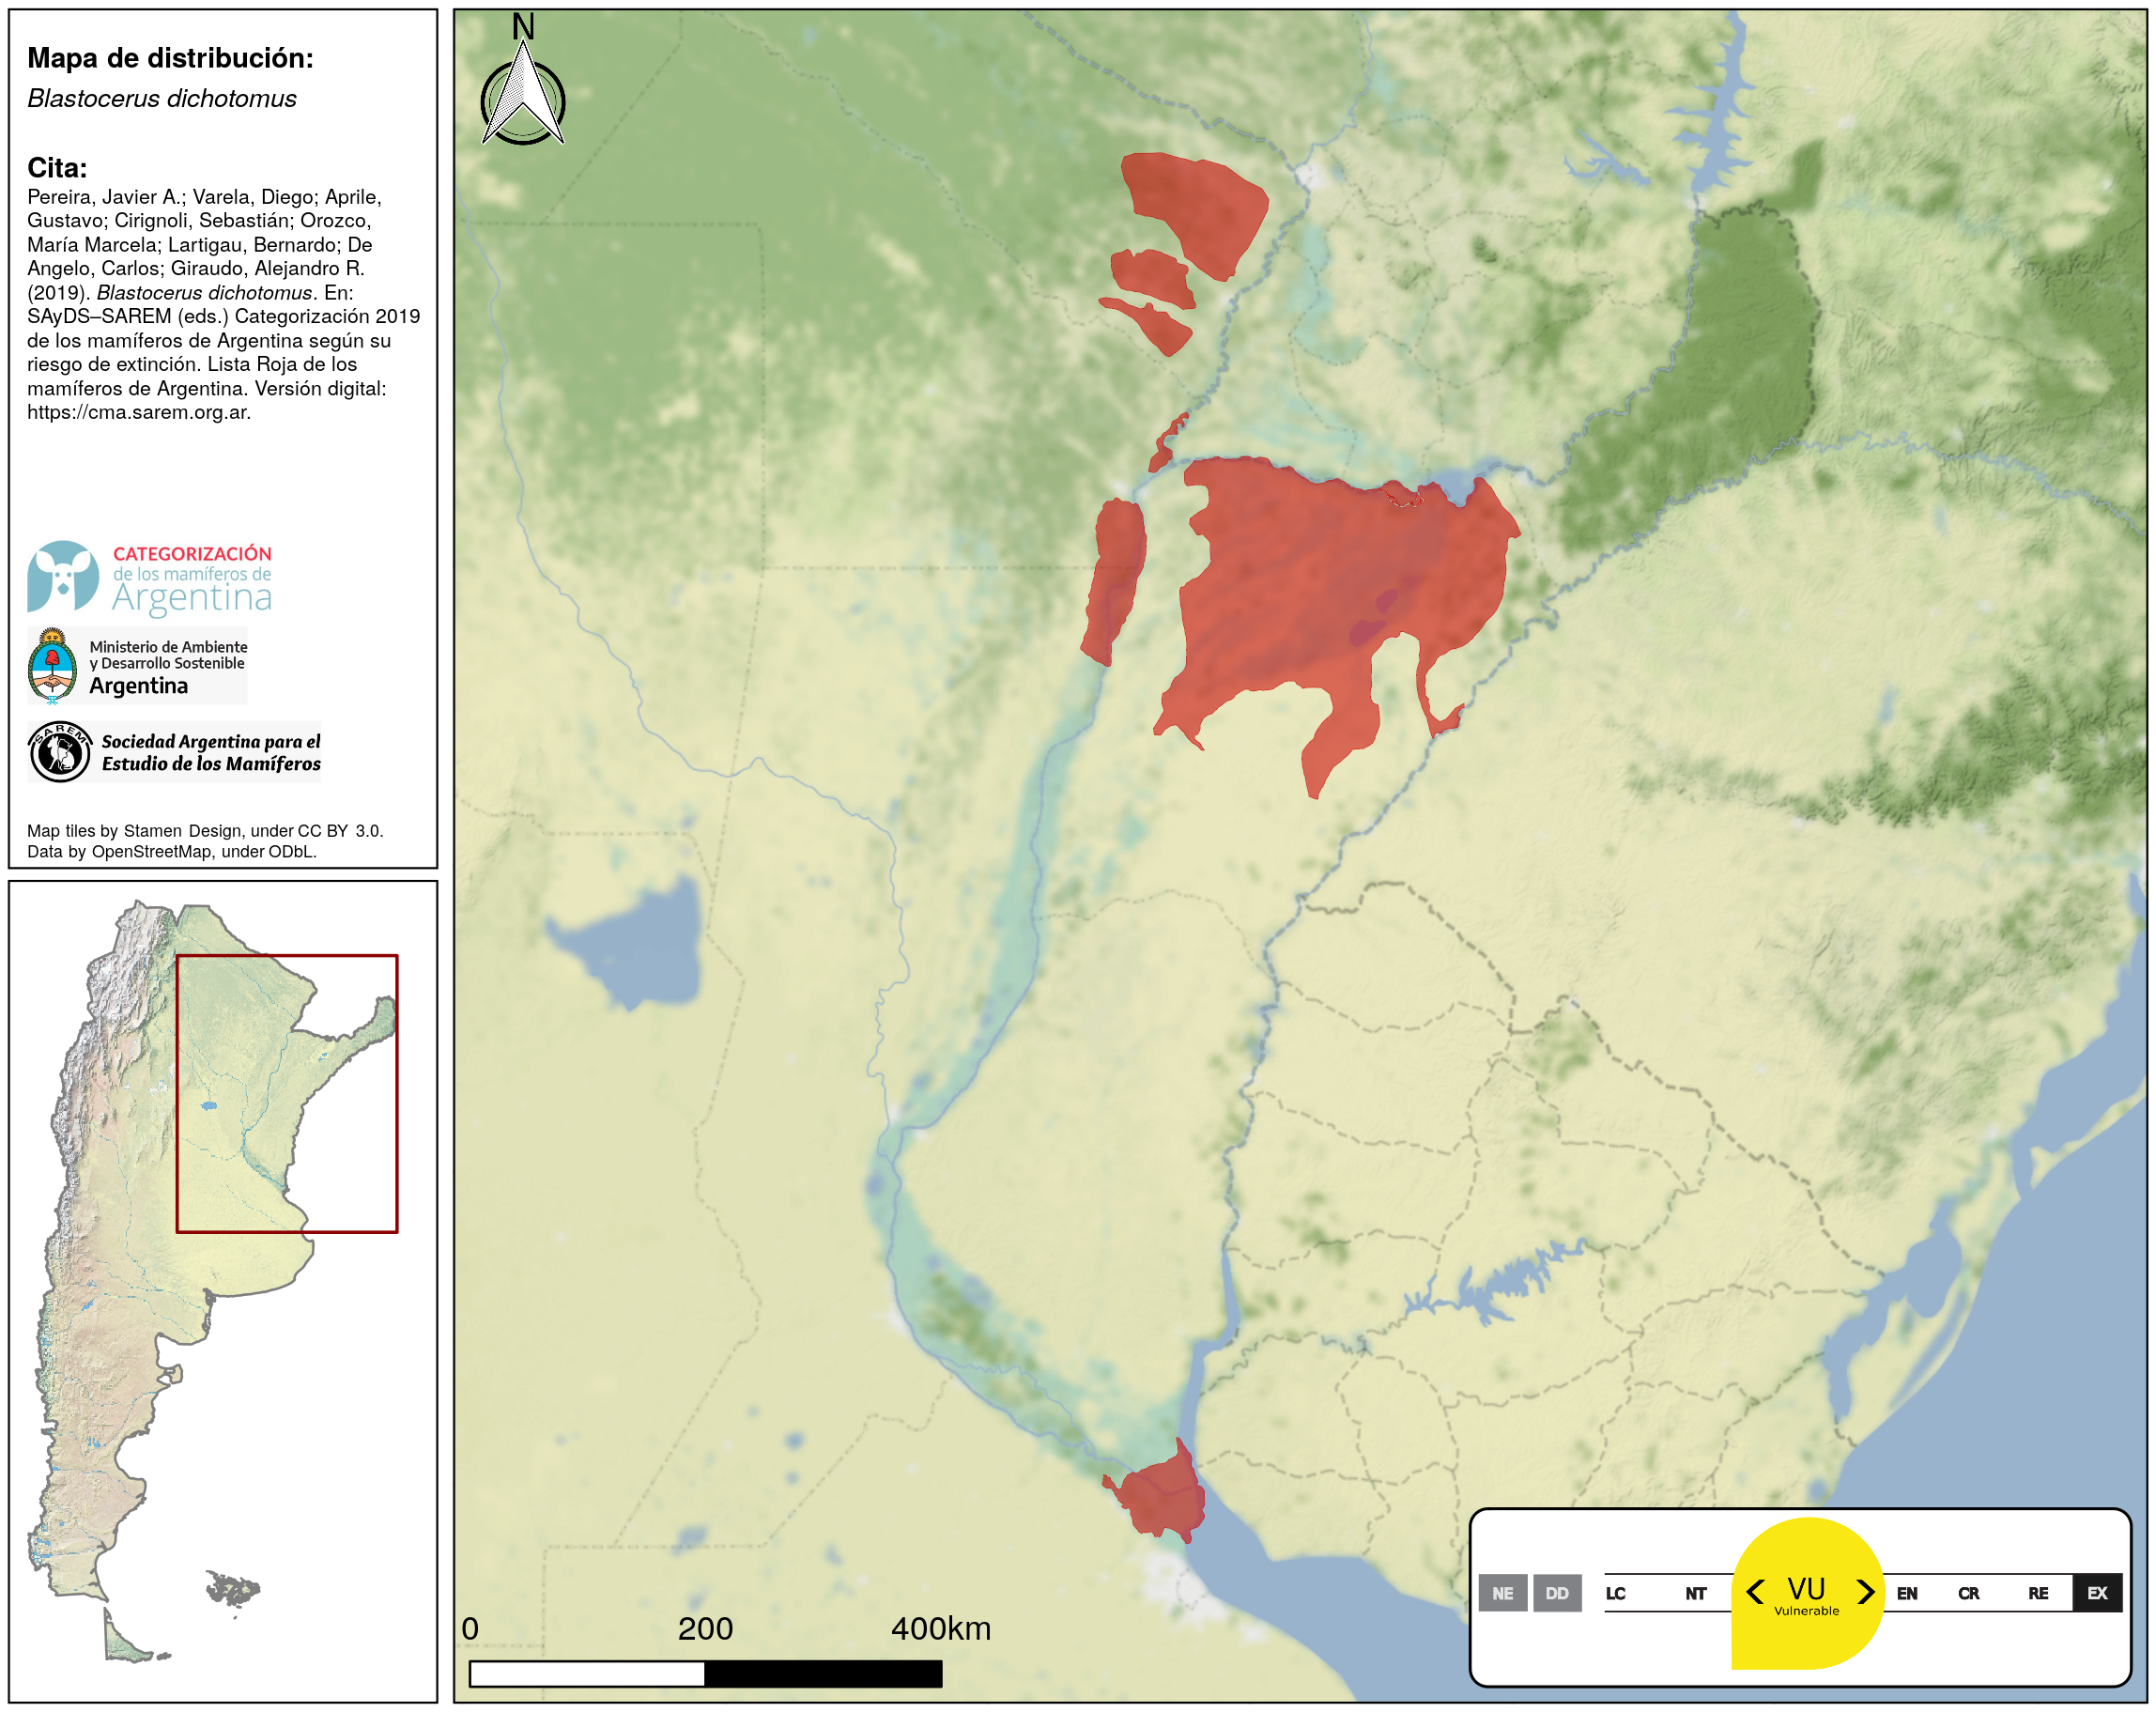
\includegraphics[width=1\linewidth]{maps/Cetartiodactyla/Blastocerus_dichotomus}

%
  \refstepcounter{section}%
  \addcontentsline{toc}{section}{\protect\numberline{\thesection}CATEGORÍAS DE CONSERVACIÓN}%
  \sectionmark{CATEGORÍAS DE CONSERVACIÓN}
\begin{table}[H]
\centering
\begin{tabular}[t]{>{\raggedright\arraybackslash}m{16cm}>{}m{16cm}}
\toprule
\cellcolor{ceil}{\textcolor{white}{\textbf{\rule{0pt}{14pt}CATEGORÍAS DE CONSERVACIÓN}}}\\
\bottomrule
\end{tabular}
\end{table}

\vspace{-0.4cm}

\textbf{Categoría Nacional de Conservación 2019}

VU (Vulnerable)

\textbf{Criterios y subcriterios}

A3cde

\textbf{Justificación de la categorización}

El ciervo de los pantanos es una especie dependiente de ambientes de
humedales y está sujeto a una alta presión de caza furtiva. Su rango de
distribución se encuentra fragmentado en al menos cuatro subpoblaciones.
Si bien la subpoblación de los Esteros del Iberá y áreas adyacentes, en
la provincia de Corrientes, ha experimentado una importante recuperación
en los últimos 30 años, el resto de las subpoblaciones se encuentran
amenazadas (ver Evaluación de Subpoblaciones). La caza furtiva y el
drenaje de los humedales para la producción agropecuaria, forestaciones
y urbanizaciones son sus principales amenazas. La especie se ve afectada
por las inundaciones extraordinarias que provocan mortalidades masivas
por aumento en la presión de cacería, desnutrición, enfermedades y
temperaturas extremas. Algunas subpoblaciones también se encuentran
amenazadas por el ataque de perros, la competencia por interferencia con
el ganado bovino y el atropellamiento en rutas. A nivel nacional, la
especie está categorizada como Vulnerable (VU) con una proyección de
reducción de su tamaño poblacional del 30\% hacia el futuro (15 años,
tres generaciones), teniendo en cuenta la reducción del EOO, AOO y la
calidad de hábitat, y los impactos de la caza furtiva y de las
inundaciones extraordinarias (incrementadas por el cambio climático).

\textbf{Evaluación de subpoblaciones locales}

\begin{tabu} to \linewidth {>{\raggedright}X>{\raggedright}X>{\raggedright}X}
\toprule
\textbf{Subpoblación} & \textbf{Categoría} & \textbf{Criterios y subcriterios}\\
\arrayrulecolor{white}
\midrule
\cellcolor{gray!6}{Esteros del Iberá y áreas aledañas} & \cellcolor{gray!6}{NT (Casi Amenazada)} & \cellcolor{gray!6}{C}\\
\bottomrule
\end{tabu}

\textbf{Justificación}

Los Esteros del Iberá y sus adyacencias albergan el mayor número de
ciervos de los pantanos de la Argentina. Durante el último relevamiento
poblacional realizado en parte de la Reserva Iberá se estimaron unos
6.000 ejemplares (De Angelo et al.~2011), mostrando una tendencia
creciente respecto a relevamientos previos en la misma área (Di Giácomo
2009) y que duplica la estimación hecha para comienzos de siglo en la
región (Soria et al.~2003). Se observa también una tendencia poblacional
en aumento en áreas satélites como el Parque Nacional Mburucuyá. Puede
inferirse una población actual superior a los 8000 individuos para la
Reserva Natural Iberá y un total de al menos 10.000 individuos maduros
para toda la región del Iberá y áreas aledañas (PN Mburucuyá, esteros
Santa Lucía, Aguapey, Miriñay, Batel y Riachuelo).

Teniendo en cuenta el número de individuos maduros, la subpoblación de
Iberá y áreas aledañas podría ser considerada Vulnerable (criterio C)
(VU), pero debe ser considerada Casi Amenazada (NT) por no cumplir con
los subcriterios correspondientes.

El estado de conservación de esta subpoblación mejoró producto de la
implementación de acciones de protección durante los últimos 30 años.
Sin embargo, el tamaño poblacional puede estar fluctuando temporalmente
debido a eventos de mortandad mayormente asociados a inundaciones
extraordinarias y condiciones climáticas adversas. Por ejemplo, en 2017
se registraron al menos 400 ciervos de los pantanos muertos (i.e., cerca
el 5\% de la población estimada en 2015), siendo el mayor episodio de
mortalidad registrado en los últimos 30 años (Orozco et al.~2013, 2017b,
2018a; Argibay et al.~2018).\vspace{0.5cm}

\begin{tabu} to \linewidth {>{\raggedright}X>{\raggedright}X>{\raggedright}X}
\toprule
\textbf{Subpoblación} & \textbf{Categoría} & \textbf{Criterios y subcriterios}\\
\arrayrulecolor{white}
\midrule
\cellcolor{gray!6}{Delta del Paraná} & \cellcolor{gray!6}{EN (En Peligro)} & \cellcolor{gray!6}{B1ac}\\
\bottomrule
\end{tabu}

\textbf{Justificación}

En los últimos 20 años, esta subpoblación mostró una tendencia creciente
en sus números, en base al incremento en el AOO, EOO y en índices de
abundancia relativa (Varela et al.~2018; Varela D. \& Lartigau B., datos
no publicados). Sin embargo, la caza furtiva (sostenida por la falta de
controles efectivos por parte de las autoridades de aplicación), la
depredación por perros y la modificación severa de los humedales para
actividades productivas, continúan presionando sobre esta población
(Varela D.,~Lartigau B.,~Fracassi N., y Pereira J., obs. pers.; Pereira
et al.~2018). Más allá de ello, el impacto más dramático sobre la
dinámica de esta población ocurre durante los períodos de inundaciones
extraordinarias, cada vez más frecuentes por el cambio climático global,
cuando varios estresores actúan en sinergia (e.g.~cacería, degradación
del hábitat, enfermedades) y generan alta mortalidad (Orozco et
al.~2017a; Varela et al.~2017; Argibay et al.~2018; Pereira et
al.~2018).

Esta subpoblación se encuentra En Peligro (EN) dado que la extensión de
presencia estimada (EOO) es menor a 2.700 km2, posee menos de 5
localidades (sensu UICN) y puede sufrir fluctuaciones extremas en el
número de individuos a causa de los efectos directos e indirectos de las
inundaciones extraordinarias.\vspace{0.5cm}

\begin{tabu} to \linewidth {>{\raggedright}X>{\raggedright}X>{\raggedright}X}
\toprule
\textbf{Subpoblación} & \textbf{Categoría} & \textbf{Criterios y subcriterios}\\
\arrayrulecolor{white}
\midrule
\cellcolor{gray!6}{Formosa} & \cellcolor{gray!6}{EN (En Peligro)} & \cellcolor{gray!6}{A4cde}\\
\bottomrule
\end{tabu}

\textbf{Justificación}

La distribución y estado de esta subpoblación no son bien conocidos dada
su escasa documentación (D'Alessio et al.~in litt.). La presencia de al
menos tres núcleos fue confirmada en base a encuestas: 1) Guaycolec -
Cañada Doce - Colonia Pastoril (departamentos Formosa y Pilcomayo); 2)
Estero Gallego - Estero González (departamentos Pirané, Laishi y
Formosa); y 3) Estero Bellaco - Estero El Alazán - Cañada Pozo de la
Suerte - Cancha Bolivia (departamentos Pirané y Laishi). El primer
núcleo es el más conocido y estable, pero la situación de los otros dos
es incierta. Además, aún persistirían dos núcleos relictuales menores en
los Esteros Ibagay (al este de la localidad de Pilagás III) y Laguna
Vera (al norte de los parajes El Paraíso y San Juan; D'Alessio et al.~in
litt).

Esta subpoblación se encuentra En Peligro (EN) dado que se estima una
reducción potencial de más del 50\% en el tamaño poblacional,
considerando el pasado cercano (10 años) y proyectado hacia el futuro
(15 años), inferido a partir de la reducción de EOO y AOO como
consecuencia de la pérdida de hábitat y la cacería.\vspace{0.5cm}

\begin{tabu} to \linewidth {>{\raggedright}X>{\raggedright}X>{\raggedright}X}
\toprule
\textbf{Subpoblación} & \textbf{Categoría} & \textbf{Criterios y subcriterios}\\
\arrayrulecolor{white}
\midrule
\cellcolor{gray!6}{Humedales del Paraná Medio (Santa Fe-Chaco-Corrientes)} & \cellcolor{gray!6}{CR (En Peligro Crítico)} & \cellcolor{gray!6}{A3cde; C1}\\
\bottomrule
\end{tabu}

\textbf{Justificación}

En Santa Fe ha desaparecido en casi toda su área de distribución
original (valle del río Paraná), donde era otrora abundante (Pautasso
2008; Eberhardt et al.~2009), quedando un pequeño núcleo remanente en el
extremo norte del sitio Ramsar ``Jaaukanigás'' (Giraudo \& Arzamendia
2008; Eberhardt et al.~2009). En base a estimaciones de densidad de la
especie obtenidas para Brasil y Corrientes, Giraudo y Arzamendia (2008)
sugirieron la existencia de entre 11 y 36 individuos en los cerca de 100
km2 de hábitat disponible para la especie. La situación actual
probablemente sea más complicada, ya que el área recibe cada vez más
turismo y los controles de cacería son muy escasos. Por su parte, en la
provincia del Chaco subsisten dos núcleos relictuales, uno sureño en
proximidades de la localidad de Basail (Departamento San Fernando), de
viabilidad incierta, y otro al norte en cercanías de la localidad de Las
Palmas (departamento Bermejo) (D'Alessio et al.~in litt). El núcleo
santafecino ya no tendría conexión con el núcleo del sur chaqueño,
aunque sí con localidades con presencia de la especie ubicadas en la
margen correntina del río Paraná (D'Alessio et al.~in litt; Giraudo A.,
obs. pers.). La cacería y la pérdida y fragmentación del hábitat siguen
ejerciendo presión sobre estos núcleos, potenciadas por la falta de
áreas protegidas. En las últimas décadas parece además haber cobrado
importancia la mortalidad durante inundaciones extraordinarias, con
recurrencias más frecuentes por el cambio climático (Giraudo \&
Arzamendia 2008).

Esta subpoblación se encuentra En Peligro Crítico (CR), con menos de 250
individuos maduros y se proyecta una reducción poblacional superior al
25\% en los próximos 5 años (1 generación) (Criterio C1) y una reducción
mayor al 80\% en las próximas 3 generaciones (Criterio A3) si se
mantienen los actuales factores de amenaza.

\textbf{Categoría Res. SAyDS 1030/04}

EP (En Peligro de Extinción)

\textbf{Categorías nacionales de conservación previas (SAREM)}

\begin{tabu} to \linewidth {>{}l>{\raggedright}X>{\raggedright}X}
\toprule
\textbf{\cellcolor{gray!6}{2012}} & \cellcolor{gray!6}{VU (Vulnerable)} & \cellcolor{gray!6}{A2}\\
\bottomrule
\end{tabu}

\begin{tabu} to \linewidth {>{}l>{\raggedright}X>{\raggedright}X}
\toprule
\textbf{\cellcolor{gray!6}{2000}} & \cellcolor{gray!6}{EN (En Peligro)} & \cellcolor{gray!6}{A1cd+2cde; B1+2; C1}\\
\bottomrule
\end{tabu}

\begin{tabu} to \linewidth {>{}l>{\raggedright}X>{\raggedright}X}
\toprule
\textbf{\cellcolor{gray!6}{1997}} & \cellcolor{gray!6}{EN (En Peligro)} & \cellcolor{gray!6}{A1cd+2cde; B1+2; C1}\\
\bottomrule
\end{tabu}

\begin{tabu} to \linewidth {>{}l>{\raggedright}X}
\toprule
\textbf{\cellcolor{gray!6}{Homologación categoría 1997}} & \cellcolor{gray!6}{EN (En Peligro)}\\
\bottomrule
\end{tabu}

\textbf{Categorías de conservación actuales en países vecinos}

\begin{tabu} to \linewidth {>{\raggedright}X>{\raggedright}X>{\raggedright}X>{\raggedright}X}
\toprule
\textbf{País} & \textbf{Categoría} & \textbf{Año} & \textbf{Cita}\\
\arrayrulecolor{white}
\midrule
\cellcolor{gray!6}{Bolivia} & \cellcolor{gray!6}{VU (Vulnerable)} & \cellcolor{gray!6}{2009} & \cellcolor{gray!6}{Aguirre et al. (2009)}\\
\bottomrule
\end{tabu}
\begin{tabu} to \linewidth {>{\raggedright}X>{\raggedright}X>{\raggedright}X>{\raggedright}X}
\toprule
\textbf{País} & \textbf{Categoría} & \textbf{Año} & \textbf{Cita}\\
\arrayrulecolor{white}
\midrule
\cellcolor{gray!6}{Brasil} & \cellcolor{gray!6}{VU (Vulnerable)} & \cellcolor{gray!6}{2018} & \cellcolor{gray!6}{ICMBio/MMA (2018)}\\
\bottomrule
\end{tabu}
\begin{tabu} to \linewidth {>{\raggedright}X>{\raggedright}X>{\raggedright}X>{\raggedright}X}
\toprule
\textbf{País} & \textbf{Categoría} & \textbf{Año} & \textbf{Cita}\\
\arrayrulecolor{white}
\midrule
\cellcolor{gray!6}{Paraguay} & \cellcolor{gray!6}{VU (Vulnerable)} & \cellcolor{gray!6}{2017} & \cellcolor{gray!6}{Cartes et al. (2017)}\\
\bottomrule
\end{tabu}
\begin{tabu} to \linewidth {>{\raggedright}X>{\raggedright}X>{\raggedright}X>{\raggedright}X}
\toprule
\textbf{País} & \textbf{Categoría} & \textbf{Año} & \textbf{Cita}\\
\arrayrulecolor{white}
\midrule
\cellcolor{gray!6}{Uruguay} & \cellcolor{gray!6}{Extinta} & \cellcolor{gray!6}{2013} & \cellcolor{gray!6}{González et al. (2013)}\\
\bottomrule
\end{tabu}

\textbf{Evaluación global UICN}

\begin{tabu} to \linewidth {>{\raggedright}X>{\raggedright}X>{\raggedright}X}
\toprule
\textbf{Año de evaluación} & \textbf{Categoría} & \textbf{Criterios y subcriterios}\\
\arrayrulecolor{white}
\midrule
\cellcolor{gray!6}{2016} & \cellcolor{gray!6}{VU (Vulnerable)} & \cellcolor{gray!6}{A4 cde}\\
\bottomrule
\end{tabu}

\arrayrulecolor{white}

%
  \refstepcounter{section}%
  \addcontentsline{toc}{section}{\protect\numberline{\thesection}TAXONOMÍA Y NOMENCLATURA}%
  \sectionmark{TAXONOMÍA Y NOMENCLATURA}
\begin{table}[H]
\centering
\begin{tabular}[t]{>{\raggedright\arraybackslash}m{16cm}>{}m{16cm}}
\toprule
\cellcolor{ceil}{\textcolor{white}{\textbf{\rule{0pt}{14pt}TAXONOMÍA Y NOMENCLATURA}}}\\
\bottomrule
\end{tabular}
\end{table}

\begin{tabu} to \linewidth {>{\raggedright\arraybackslash}p{6cm}>{\raggedright\arraybackslash}p{1cm}>{\raggedright}X}
\toprule
\textbf{\cellcolor{gray!6}{Orden}} & \cellcolor{gray!6}{} & \cellcolor{gray!6}{Cetartiodactyla}\\
\bottomrule
\end{tabu} \vspace{0.3cm}
\begin{tabu} to \linewidth {>{\raggedright\arraybackslash}p{6cm}>{\raggedright\arraybackslash}p{1cm}>{\raggedright}X}
\toprule
\textbf{\cellcolor{gray!6}{Familia}} & \cellcolor{gray!6}{} & \cellcolor{gray!6}{Cervidae}\\
\bottomrule
\end{tabu} \vspace{0.3cm}
\begin{tabu} to \linewidth {>{\raggedright\arraybackslash}p{6cm}>{\raggedright\arraybackslash}p{1cm}>{\raggedright}X}
\toprule
\textbf{\cellcolor{gray!6}{Nombre científico}} & \cellcolor{gray!6}{} & \cellcolor{gray!6}{\textit{Blastocerus dichotomus} (Illiger, 1815)}\\
\bottomrule
\end{tabu} \vspace{0.3cm}
\begin{tabu} to \linewidth {>{\raggedright\arraybackslash}p{6cm}>{\raggedright\arraybackslash}p{1cm}>{\raggedright}X}
\toprule
\textbf{\cellcolor{gray!6}{Nombre común}} & \cellcolor{gray!6}{} & \cellcolor{gray!6}{Ciervo de los pantanos}\\
\bottomrule
\end{tabu} \vspace{0.3cm}
\begin{tabu} to \linewidth {>{\raggedright\arraybackslash}p{6cm}>{\raggedright\arraybackslash}p{1cm}>{\raggedright}X}
\toprule
\textbf{\cellcolor{gray!6}{Nombres comunes locales}} & \cellcolor{gray!6}{} & \cellcolor{gray!6}{Guazú pucú (guaraní)}\\
\textbf{} &  & Epelve (mocoví)\\
\textbf{\cellcolor{gray!6}{}} & \cellcolor{gray!6}{} & \cellcolor{gray!6}{Calimgo (qom)}\\
\textbf{} &  & Huasé\\
\textbf{\cellcolor{gray!6}{}} & \cellcolor{gray!6}{} & \cellcolor{gray!6}{iwase o wase (wichi)}\\
\bottomrule
\end{tabu} \vspace{0.3cm}
\begin{tabu} to \linewidth {>{\raggedright\arraybackslash}p{6cm}>{\raggedright\arraybackslash}p{1cm}>{\raggedright}X}
\toprule
\textbf{\cellcolor{gray!6}{Nombres comunes en inglés}} & \cellcolor{gray!6}{} & \cellcolor{gray!6}{Marsh Deer}\\
\bottomrule
\end{tabu} \vspace{0.3cm}
\begin{tabu} to \linewidth {>{\raggedright\arraybackslash}p{6cm}>{\raggedright\arraybackslash}p{1cm}>{\raggedright}X}
\toprule
\textbf{\cellcolor{gray!6}{Nombres comunes en portugués}} & \cellcolor{gray!6}{} & \cellcolor{gray!6}{Cervo-do-pantanal}\\
\textbf{} &  & Suaçuapara\\
\textbf{\cellcolor{gray!6}{}} & \cellcolor{gray!6}{} & \cellcolor{gray!6}{Guaçupuçu}\\
\bottomrule
\end{tabu} \vspace{0.3cm}

\textbf{Comentarios taxonómicos}

Único representante del género \textit{Blastocerus}. No se han propuesto
subespecies.

\arrayrulecolor{white}

%
  \refstepcounter{section}%
  \addcontentsline{toc}{section}{\protect\numberline{\thesection}INFORMACIÓN RELEVANTE PARA LA EVALUACIÓN}%
  \sectionmark{INFORMACIÓN RELEVANTE PARA LA EVALUACIÓN}
\begin{table}[H]
\centering
\begin{tabular}[t]{>{\raggedright\arraybackslash}m{16cm}>{}m{16cm}}
\toprule
\cellcolor{ceil}{\textcolor{white}{\textbf{\rule{0pt}{14pt}INFORMACIÓN RELEVANTE PARA LA EVALUACIÓN}}}\\
\bottomrule
\end{tabular}
\end{table}

%
  \refstepcounter{section}%
  \addcontentsline{toc}{section}{\protect\numberline{\thesection}RANGO GEOGRÁFICO, OCURRENCIA Y ABUNDANCIA}%
  \sectionmark{RANGO GEOGRÁFICO, OCURRENCIA Y ABUNDANCIA}
\begin{table}[H]
\centering
\begin{tabular}[t]{>{\raggedright\arraybackslash}m{16cm}>{}m{16cm}}
\toprule
\cellcolor{ceil}{\textcolor{white}{\textbf{\rule{0pt}{14pt}RANGO GEOGRÁFICO, OCURRENCIA Y ABUNDANCIA}}}\\
\bottomrule
\end{tabular}
\end{table}

\textbf{Presencia en el territorio nacional:} residente

\textbf{Comentarios sobre la distribución actual e histórica}

Antiguamente extendida por buena parte del área subtropical y templada
húmeda del país, hoy se encuentra reducida a poblaciones aisladas (la
mayoría de ellas pequeñas) en las zonas de esteros y lagunas asociadas a
las cuencas de los ríos Paraná y Paraguay: este de Formosa, centro,
norte, noreste y oeste de Corrientes, extremo noreste de Santa Fe,
sudeste de Chaco, y el bajo delta bonaerense y entrerriano (incluyendo
el extremo sur del río Uruguay). Existen registros históricos para la
provincia de Salta, en inmediaciones del río Pilcomayo y áreas inundadas
en la frontera con Bolivia y Paraguay, y en el área de influencia del
río Bermejo (Díaz et al.~2000). También existen registros históricos
para la provincia de Misiones, en los departamentos de Apóstoles, San
Ignacio y Capital (Massoia et al.~2006). Es probable que la especie
estuviera extendida en todo el Chaco oriental, existiendo registros en
sitios arqueológicos de la región (Santini \& Plischuk 2006; Santini
2009).

\begin{tabu} to \linewidth {>{\raggedright\arraybackslash}p{8cm}>{\raggedright\arraybackslash}p{0.5cm}>{\raggedright}X}
\toprule
\textbf{\cellcolor{gray!6}{Presencia confirmada por provincia:}} & \cellcolor{gray!6}{} & \cellcolor{gray!6}{Buenos Aires}\\
\textbf{} &  & Chaco\\
\textbf{\cellcolor{gray!6}{}} & \cellcolor{gray!6}{} & \cellcolor{gray!6}{Corrientes}\\
\textbf{} &  & Entre Ríos\\
\textbf{\cellcolor{gray!6}{}} & \cellcolor{gray!6}{} & \cellcolor{gray!6}{Formosa}\\
\textbf{} &  & Santa Fe\\
\bottomrule
\end{tabu}

\begin{tabu} to \linewidth {>{\raggedright\arraybackslash}p{8cm}>{\raggedright\arraybackslash}p{0.5cm}>{\raggedright}X}
\toprule
\textbf{\cellcolor{gray!6}{Presencia en ecorregiones de Argentina:}} & \cellcolor{gray!6}{} & \cellcolor{gray!6}{Chaco Húmedo}\\
\textbf{} &  & Esteros del Iberá\\
\textbf{\cellcolor{gray!6}{}} & \cellcolor{gray!6}{} & \cellcolor{gray!6}{Delta e Islas del Paraná}\\
\textbf{} &  & Espinal\\
\textbf{\cellcolor{gray!6}{}} & \cellcolor{gray!6}{} & \cellcolor{gray!6}{Campos y Malezales}\\
\bottomrule
\end{tabu}

\begin{tabu} to \linewidth {>{\raggedright\arraybackslash}p{8cm}>{\raggedright\arraybackslash}p{0.5cm}>{\raggedright}X}
\toprule
\textbf{\cellcolor{gray!6}{Presencia en ecorregiones globales terrestres:}} & \cellcolor{gray!6}{} & \cellcolor{gray!6}{ID571 – Chaco Húmedo}\\
\textbf{} &  & ID575 – Espinal\\
\textbf{\cellcolor{gray!6}{}} & \cellcolor{gray!6}{} & \cellcolor{gray!6}{ID585 – Sabana Inundada del Paraná}\\
\textbf{} &  & ID586 – Sabanas Mesopotámicas del Cono Sur\\
\bottomrule
\end{tabu}

\begin{tabu} to \linewidth {>{\raggedright}X>{\raggedright}X>{\raggedright}X}
\toprule
\textbf{Patrón de distribución} & \textbf{Cantidad de localidades} & \textbf{Rango altitudinal}\\
\midrule
\cellcolor{gray!6}{discontinuo/fragmentado} & \cellcolor{gray!6}{12} & \cellcolor{gray!6}{0-100 msnm}\\
\bottomrule
\end{tabu}

\arrayrulecolor{white}

%
  \refstepcounter{section}%
  \addcontentsline{toc}{section}{\protect\numberline{\thesection}DATOS MORFOMÉTRICOS}%
  \sectionmark{DATOS MORFOMÉTRICOS}
\begin{table}[H]
\centering
\begin{tabular}[t]{>{\raggedright\arraybackslash}m{16cm}>{}m{16cm}}
\toprule
\cellcolor{ceil}{\textcolor{white}{\textbf{\rule{0pt}{14pt}DATOS MORFOMÉTRICOS}}}\\
\bottomrule
\end{tabular}
\end{table}

\begin{tabu} to \linewidth {>{\raggedright}X>{\raggedright}X>{\raggedright}X}
\toprule
\textbf{Peso} & \textbf{Peso de la hembra} & \textbf{Peso del macho}\\
\midrule
\cellcolor{gray!6}{80-140 kg} & \cellcolor{gray!6}{80-100 kg} & \cellcolor{gray!6}{90-140 kg}\\
\bottomrule
\end{tabu}
\arrayrulecolor{white}

%
  \refstepcounter{section}%
  \addcontentsline{toc}{section}{\protect\numberline{\thesection}RASGOS ETO-ECOLÓGICOS}%
  \sectionmark{RASGOS ETO-ECOLÓGICOS}
\begin{table}[H]
\centering
\begin{tabular}[t]{>{\raggedright\arraybackslash}m{16cm}>{}m{16cm}}
\toprule
\cellcolor{ceil}{\textcolor{white}{\textbf{\rule{0pt}{14pt}RASGOS ETO-ECOLÓGICOS}}}\\
\bottomrule
\end{tabular}
\end{table}

%
  \refstepcounter{section}%
  \addcontentsline{toc}{section}{\protect\numberline{\thesection}CONSERVACIÓN E INVESTIGACIÓN}%
  \sectionmark{CONSERVACIÓN E INVESTIGACIÓN}
\begin{table}[H]
\centering
\begin{tabular}[t]{>{\raggedright\arraybackslash}m{16cm}>{}m{16cm}}
\toprule
\cellcolor{ceil}{\textcolor{white}{\textbf{\rule{0pt}{14pt}CONSERVACIÓN E INVESTIGACIÓN}}}\\
\bottomrule
\end{tabular}
\end{table}

\textbf{La especie ¿está presente en áreas naturales protegidas?:} sí

\textbf{Presencia de la especie en áreas naturales protegidas}

Parque Nacional Mburucuyá (Corrientes), Parque Nacional (en formación)
Iberá (Corrientes), Parque Nacional Ciervo de los Pantanos (ex Reserva
Natural Otamendi; Buenos Aires), Parque y Reserva Natural Provincial
Iberá (Corrientes), Reserva de Biosfera Delta del Paraná (Buenos Aires),
Sitio RAMSAR Humedales Chaco (Chaco), Sitio RAMSAR Jaaukanigás (Santa
Fe), Reserva Natural Rincón de Santa María (Corrientes), Reserva Privada
El Bagual (Formosa) y Reserva Privada Estancia Guaycolec (Formosa).

Extinta en los parques nacionales Pre Delta (Entre Ríos), Chaco (Chaco)
y Río Pilcomayo (Formosa) (Heinonen Fortabat \& Chebez 1997; SIB 2018).

\textbf{Marco legal de la especie}

Especie declarada ``Monumento Natural Provincial'' en las provincias de
Corrientes (Decreto 1.555/1992), Chaco (Ley 4.306/1996), Buenos Aires
(Ley 12.209/1998) y Entre Ríos (Res. DGRN 852/2015). Declarada ``En
peligro de extinción'' mediante Res. 1.030/04 de la Secretaría de
Ambiente de la Nación e incluida en el Apéndice I de la Convención
CITES.

\textbf{Planes de acción y/o proyectos de conservación o manejo
actuales}

En 1995 se puso en marcha el ``Proyecto Ciervo de los Pantanos'' de la
Asociación para la Conservación y el Estudio de la Naturaleza
(PCP/ACEN), focalizado en estudiar la distribución, abundancia relativa
y amenazas del ciervo en el Delta del Paraná (Varela 2003; D'Alessio et
al.~2006; D'Alessio 2016; D'Alessio et al., in litt). Desde ese proyecto
se impulsaron esfuerzos interinstitucionales para su conservación in
situ que finalizaron con la creación de la Reserva de Biosfera ``Delta
del Paraná''. El PCP/ACEN trabajó en el área hasta 2012, pero varias de
sus líneas de trabajo fueron luego continuadas por el ``Proyecto
Pantano'', una iniciativa multisectorial (i.e., CONICET, INTA, ACEN,
productores forestales) lanzada en 2015 (Pereira et al.~2018b). Este
proyecto apunta a conocer la ecología espacial, ecología nutricional,
genética poblacional y evolución de la distribución y abundancia del
ciervo de los pantanos en el Delta, complementados con actividades de
educación ambiental, comunicación y gestión para la conservación. Entre
estas últimas, cabe destacar el impulso que se dio a la creación, en
2018, del Parque Nacional Ciervo de los Pantanos (Buenos Aires).

En el año 2007 empezaron a investigarse eventos de mortalidad de la
especie en Corrientes (Orozco et al.~2013, 2018b). Para 2016 se logró
consolidar un proyecto en el que contribuyen investigadores del CONICET,
INTA, UBA y SENASA, abocado al estudio sanitario de la especie con foco
en los eventos de mortalidad. Como parte de la iniciativa se desarrolló
una red de alerta temprana de casos (Orozco et al.~2018a, 2018b), con
participación del personal de áreas protegidas nacionales y
provinciales.

\textbf{Experiencias de reintroducción o erradicación:} sí

Existió un proyecto por parte de la APN (1997) para reintroducir la
especie en el Parque Nacional Pilcomayo (Formosa) a partir de individuos
obtenidos durante la operación de rescate de fauna en Porto Primavera,
Brasil. Sin embargo, el mismo fue desestimado luego de constatarse que
los individuos candidatos a translocar mostraban altos índices de
positividad serológica para agentes infecto-contagiosos (D'Alessio et
al., in litt). En la actualidad, dos iniciativas buscan reintroducir al
ciervo de los pantanos en áreas protegidas nacionales: Parque Nacional
Pre Delta (Alonso J., com. pers. 2017) y Parque Nacional El Impenetrable
(Di Martino S., com. pers., 2018).

Por otro lado, la provincia de Buenos Aires creó en 2008 el Comité
Científico-Técnico Ciervo de los Pantanos, liderado desde el OPDS e
integrado por diversas instituciones (CONICET, INTA, ACEN, Fundación
Temaiken, Administración de Parques Nacionales, Fundación Azara, Arauco
S.A., Municipio de San Fernando, entre otras) cuyo objetivo es el
abordaje de las problemáticas de conservación que enfrenta la especie en
la región, y cuyas acciones están relacionadas con el~ rescate,
rehabilitación y reinserción al delta de individuos hallados heridos,
enfermos o víctimas de tenencia ilegal (Vázquez et al.~2018).

\textbf{Rol ecológico / servicios ecosistémicos}

La especie puede considerarse como un buen indicador del estado de
conservación de los humedales a escala de paisaje, ya que es sensible a
la caza furtiva y dependiente de ecosistemas particulares, como los
embalsados.

Si bien en otras áreas de su distribución en Sudamérica, la especie
puede ser considerada presa de grandes depredadores como el yaguareté,
en las áreas de distribución actual, su principal depredador natural ha
desaparecido.

\textbf{Necesidades de investigación y conocimiento}

Es necesario contar con un plan nacional de manejo de la especie,
iniciativa que aún no pudo ser concretada pese a los esfuerzos iniciados
durante el ``Primer Taller Nacional para el Diagnóstico del Estado de
Situación del Ciervo de los Pantanos'', realizado en agosto de 2009 en
Santa Fe. El documento final resultante de ese taller contiene un
análisis detallado de las necesidades de investigación y acciones de
manejo para cada subpoblación. Como proyectos prioritarios requeridos en
la actualidad, pueden destacarse la necesidad de obtener líneas de base
(p.e., abundancia poblacional, estructura demográfica, sanidad) para
diseñar programas de monitoreo para todas las subpoblaciones; el
modelado de los efectos del incremento en la frecuencia de inundaciones
extraordinarias como insumo para proponer estrategias de adaptación al
cambio global; el monitoreo de la salud de las poblaciones a la luz del
avance de la ganadería y la degradación de los humedales; y la obtención
de información demográfica para modelar la dinámica de las poblaciones
(fundamentalmente Iberá y Delta del Paraná) en función de los eventos
recurrentes de mortalidad masiva y el cambio global.

%
  \refstepcounter{section}%
  \addcontentsline{toc}{section}{\protect\numberline{\thesection}BIBLIOGRAFÍA}%
  \sectionmark{BIBLIOGRAFÍA}
\begin{table}[H]
\centering
\begin{tabular}[t]{>{\raggedright\arraybackslash}m{16cm}>{}m{16cm}}
\toprule
\cellcolor{ceil}{\textcolor{white}{\textbf{\rule{0pt}{14pt}BIBLIOGRAFÍA}}}\\
\bottomrule
\end{tabular}
\end{table}

\setlength{\parindent}{20pt}\noindent\textbf{LITERATURA CITADA}

AGUIRRE, L. F., R. AGUAYO, J. BALDERRAMA, C. CORTEZ, \& T. TARIFA.
(EDS). 2009. Libro rojo de la fauna silvestre de vertebrados de Bolivia.
Ministerio de Medio Ambiente y Agua. La Paz

ANDRIOLO, A., M. J. R. COSTA, U. PIOVEZAN, \& J. M. B. DUARTE. 2005.
Aerial line transect survey to estimate abundance of marsh deer
(\textit{Blastocerus} \textit{dichotomus}) (Illiger, 1815). Brazilian
Archives of Biology and Technology 48:807‒814.

ARGIBAY, H., L. RODRÍGUEZ PLANES, P. RODRÍGUEZ, \& M. M. OROZCO. 2018.
Inundaciones como factor determinante en eventos de mortalidad de
\textit{Blastocerus} \textit{dichotomus} en dos poblaciones de
Argentina. XIII Congreso Internacional de Manejo de Fauna Silvestre en
la Amazonía y Latinoamérica, Libro de Resúmenes.

BALBUENA, P. J. ET AL. 2015. Atropellamiento de mamíferos silvestres
amenazados de extinción en la Ruta Nacional 12, al norte de la provincia
de Corrientes. Un problema para la conservación de la fauna silvestre y
la seguridad vial. Dirección de Fauna y Flora, y Dirección de Recursos
Naturales, Santa Fe.

BECCACECI, M. D. 1994. Parasites of the marsh deer, \textit{Blastocerus}
\textit{dichotomus}, in the wild. IUCN‒SSC Veterinary Group Newsletter.
Gland, Switzerland.

D'ALESSIO, S. 2016. Evaluación de la presencia de embalsados en las
islas del Bajo Delta del Paraná y su importancia para el Ciervo de los
Pantanos (\textit{Blastocerus} \textit{dichotomus}) en períodos de
inundación. Tesis de Licenciatura. Universidad de Buenos Aires, Buenos
Aires, Argentina.

CARTES, J. L. ET AL. 2017. Cetartiodactyla y Perissodactyla : animales
con pezuñas. Libro Rojo de los Mamíferos del Paraguay: especies
amenazadas de extinción (S. Saldívar, V. Rojas \& D. Giménez, eds.).
Libro Rojo de los Mamíferos del Paraguay: especies amenazadas de
extinción. Asociación Paraguaya de Mastozoología y Secretaría del
Ambiente. Editorial CREATIO, Asunción.

D'ALESSIO, S., B. LARTIGAU, G. APRILE, P. HERRERA, \& D. VARELA. 2006.
Distribución, abundancia relativa y acciones para la conservación del
ciervo de los pantanos en el bajo Delta del río Paraná. Humedales
Fluviales de América del Sur. Hacia un manejo sustentable (J. Peteán \&
J. Cappato, comps.). PROTEGER Ediciones, Santa Fé.

D'ALESSIO, S. ET AL. In litt. Ciervo de los Pantanos
\textit{Blastocerus} \textit{dichotomus} (Illiger, 1815). Manejo de
fauna silvestre en la Argentina. Programa de Conservación de Especies
Amenazadas. MAyDS y FHN Félix de Azara, Buenos Aires.

DE ANGELO, C. D., A. S. DI GIÁCOMO, \& I. JIMÉNEZ PÉREZ. 2011. Situación
poblacional del ciervo de los pantanos \textit{Blastocerus}
\textit{dichotomus} en los Esteros del Iberá. XXIV Jornadas Argentinas
de Mastozoología, Libro de Resúmenes.

DEBÁRBORA, V. N., S. NAVA, S. CIRIGNOLI, A. A. GUGLIELMONE, \& A. S.
POI. 2012. Ticks (Acari: Ixodidae) parasitizing endemic and exotic wild
mammals in the Esteros del Iberá wetlands, Argentina. Systematic and
Applied Acarology 17:243‒250.

DI GIACOMO, A. 2009. Abundancia y distribución actual de la macrofauna
del Iberá y posibles escenarios futuros ante el cambio climático.
Laboratorio de Ecología del Comportamiento Animal, Universidad de Buenos
Aires, Argentina. Informe sin publicar.

DÍAZ, M. M., J. K. BRAUN, M. A. MARES, \& R. M. BARQUEZ. 2000. An update
of the taxonomy, systematics, and distribution of the mammals of Salta
province, Argentina. Occasional Papers of the Sam Noble Oklahoma Museum
of Natural History 10:1‒52.

EBERHARDT, A., L. ANTONIAZZI, A. KEES, P.HERRERA, B. LARTIGAU, \& S.
D´ALESSIO. 2009. Distribución y conservación del Ciervo de los Pantanos
(\textit{Blastocerus} \textit{dichotomus}) en la provincia de Santa Fe,
Argentina. Resultados Preliminares. BIOLÓGICA Nro 10. Museo Provincial
de Ciencias Naturales ``Florentino Ameghino'', Santa Fe.

FERGNANI, D., N. FRACASSI, R. QUINTANA \& J. A. PEREIRA. 2017. Efecto
del ganado sobre la abundancia relativa de las especies de medianos y
grandes mamíferos del Bajo Delta del Río Paraná. XXX Jornadas Argentinas
de Mastozoología, Libro de Resúmenes.

GIRAUDO, A. R., \& V. ARZAMENDIA. 2008. Registro actual de una especie
amenazada \textit{Blastocerus} \textit{dichotomus} (Illiger, 1815) en el
Sitio Ramsar Jaaukanigás (Santa Fe, Argentina) y análisis de su estado
de conservación en el río Paraná. FABICIB 12: 91‒102.

GÓMEZ, H., \& B. RÍOS‒UZEDA. 2004. Abundancia y distribución del ciervo
de los pantanos (\textit{Blastocerus} \textit{dichotomus}) en las Pampas
del Heath (PN Madidi, La Paz, Bolivia). Wildlife Conservation Society --
Bolivia. Living Landscapes Program. Technical report.

GONZÁLEZ, E. M., J. A. MARTÍNEZ-LANFRANCO, E. JURI, A. L. RODALES, G.
BOTTO, A. SOUTULLO. 2013. \textit{Blastocerus} \textit{dichotomus}. Base
de datos de especies.
\url{https://www.dinama.gub.uy/especies/especie/B_dichotom/}

GUERISOLI, M., O. GALLO, \& J. A. PEREIRA. 2018. Daño por ciervos en
sistemas agrícola-forestales: una revisión bibliográfica de métodos para
reducir/evitar el impacto en vista a su aplicación en el Delta del
Paraná. XXXI Jornadas Argentinas de Mastozoología, Libro de Resúmenes.

HEINONEN FORTABAT, S. \& J. C. CHEBEZ. 1997. Los mamíferos de los
Parques Nacionales de la Argentina. Monografía Especial LOLA 14, Buenos
Aires.

ICMBio/MMA. 2018. Livro Vermelho da Fauna Brasileira Ameaçada de
Extinção: Volume I. 1ra. ed.~Brasília, DF.

IEZZI, M. E., N. G. FRACASSI, \& J. A. PEREIRA. 2017. Conservation of
the largest cervid of South America: interactions between people and the
Vulnerable marsh deer \textit{Blastocerus} \textit{dichotomus}. Oryx
52:654‒660

MARQUEZ, A., J. MALDONADO, S. GONZALEZ, M. BECCACECI, J. E. GARCIA, \&
J. M. B. DUARTE. 2006. Phylogeography and pleistocene demographic
history of the endangered marsh deer (\textit{Blastocerus}
\textit{dichotomus}) from the Rio de la Plata basin. Conservation
genetics 7:563‒575.

MASSOIA, E., J. C. CHEBEZ, \& A. BOSSO. 2006. Los mamíferos silvestres
de la provincia de Misiones, Argentina. Edición de los autores, Buenos
Aires.

MAURO, R. A., G. M. MOURÃO, M. PEREIRA DA SILVA, M. E. COUTINHO, W. M.
TOMAS, \& W. E. MAGNUSSON. 1995. Influência do hábitat na densidade e
distribuição de cervo (\textit{Blastocerus} \textit{dichotomus}) durante
a estação de seca no pantanal Mato‒Grossense. Revista Brasilera de
Biología 55:745‒751.

OROZCO, M. M., C. MARULL, I. JIMÉNEZ PÉREZ, \& R. GÜRTLER. 2013.
Mortalidad invernal de ciervo de los pantanos (\textit{Blastocerus}
\textit{dichotomus}) en humedales del Noreste de Argentina.
Mastozoologia Neotropical 20:163‒170.

OROZCO, M. M. ET AL. 2017a. El Proceso de inundación de la Cuenca del
Rio Paraná: Implicancias en la salud de las poblaciones de ciervo de los
pantanos. 10° Jornadas Internacionales de Veterinaria Práctica, Libro de
Resúmenes.

OROZCO, M. M., H. D. ARGIBAY, P. F. RODRÍGUEZ, \& L. I. RODRÍGUEZ
PLANES. 2017b. El evento de inundación extraordinaria en Corrientes,
Argentina durante 2017: impacto en las poblaciones de ciervo de los
pantanos (\textit{Blastocerus} \textit{dichotomus}). XXX Jornadas
Argentinas de Mastozoología, Libro de Resúmenes.

OROZCO, M. M. ET AL. 2018a. Situación actual de \textit{Blastocerus}
\textit{dichotomus} en Argentina - reseña sobre episodios de mortalidad.
XIII Congreso Internacional de Manejo de Fauna Silvestre en la Amazonía
y Latinoamérica, Libro de Resúmenes.

OROZCO, M. M. ET AL. 2018b. Abordaje integral de los episodios de
mortalidad de \textit{Blastocerus} \textit{dichotomus}: generando redes
de trabajo. XIII Congreso Internacional de Manejo de Fauna Silvestre en
la Amazonía y Latinoamérica, Libro de Resúmenes.

PACIFICI, M. ET AL. 2013. Generation length for mammals. Nature
Conservation 5:8--94.

PAUTASSO, A. A. 2008. Mamíferos de la provincia de Santa Fe, Argentina.
Comunicaciones del Museo Provincial de Ciencias Naturales ``Florentino
Amerghino''. 13:1‒248.

PEREIRA, J. A., D. M. VARELA, B. LARTIGAU, \& N. FRACASSI. 2018a.
``Puntos calientes'' de mortalidad del ciervo de los pantanos
\textit{Blastocerus} \textit{dichotomus} durante la inundación
extraordinaria de 2016 en el Delta del Paraná. XXXI Jornadas Argentinas
de Mastozoología, Libro de Resúmenes.

PEREIRA, J. A. ET AL. 2018b. Introducing the ``Pantano Project'' to
conserve the southernmost population of the marsh deer. Deer Specislist
Group News 30:15‒21.

PINDER, L. 1996. Marsh deer \textit{Blastocerus} \textit{dichotomus}
population estimate in the Paraná River, Brasil. Biological
Conservation. 75:87--91.

POLEGATO, B. F., E. D. S. ZANETTI, \& J. M.B. DUARTE. 2018. Monitoring
ovarian cycles, pregnancy and post-partum in captive marsh deer
(\textit{Blastocerus} \textit{dichotomus}) by measuring fecal steroids.
Conservation Physiology 6:cox073.

RAMOS, H. G. C. 2004. O ciclo do chifre do cervo-do pantanal: aspectos
ecológicos e reprodutivos. Tesis de Maestría. FCAV/UNESP, Jaboticabal,
San Pablo, Brasil.

RIOS-UZEDA, B. 2008. Estimativa populacional, seleção de habitat,
distribuição e conservação do cervo‒do‒pantanal nas savanas do norte da
Bolívia. Tesis de Maestría. Universidade Federal do Mato Groso do Sul,
UFMS, Campo Grande, Mato Groso do Sul, Brasil.

SACCHI, A. B., J. M. B. DUARTE, M. R. ANDRE, \& R. Z MACHADO. 2012.
Prevalence and molecular characterization of Anaplasmataceae agents in
free‒ranging Brazilian marsh deer (\textit{Blastocerus}
\textit{dichotomus}). Comparative Immunology, Microbiology \& Infectious
Diseases 35:325‒334.

SANTINI, M. 2009. Prehistoria de la región meridional del Gran Chaco:
aportes del análisis de restos faunísticos en la reconstrucción de las
estrategias adaptativas de los grupos aborígenes durante el Holoceno
tardío. Tesis de Doctorado. Universidad Nacional de La Plata, La Plata,
Argentina.

SANTINI, M., \& M. PLISCHUK. 2006. Sector Ribereño Paraguay‒Paraná:
análisis de los conjuntos de artefactos óseos provenientes de dos sitios
arqueológicos. Actas del XXVI Encuentro de Geohistoria Regional,
pp.~491‒495.

SCHALLER, G. B., \& J. M. C. VASCONCELOS. 1978. A marsh deer census in
Brazil (\textit{Blastocerus} \textit{dichotomus}). Oryx 14:345‒351.

SIB. 2018. Sistema de Información de Biodiversidad de la Administración
de Parques Nacionales.

SORIA, A., S. HEINONEN FORTABAT, \& S. FABRI. 2003. Estimación
poblacional de ciervo de los pantanos en los Esteros del Iberá,
Corrientes, Argentina. Fauna del Iberá (B. Alvarez, ed.). Universidad
Nacional del Nordeste, Corrientes.

SZABÓ, M. P. J., M. B. LABRUNA, M. C. PEREIRA, \& J. M. B. DUARTE. 2003.
Ticks (Acari: Ixodidae) on wild marsh‒deer (\textit{Blastocerus}
\textit{dichotomus}) from southeast Brazil: infestations before and
after habitat loss. Journal of Medical Entomology 40:268‒274.

TOMAS, W. M., S. M. SALIS, M. P. SILVA, \& G. MOURÃO. 2001. Marsh deer
(\textit{Blastocerus} \textit{dichotomus}) distribution as a function of
floods in the Pantanal wetland, Brazil. Studies on Neotropical Fauna and
Environment 36:9‒13.

VARELA, D. 2003. Distribución, Abundancia y Conservación del Ciervo de
los Pantanos (\textit{Blastocerus} \textit{dichotomus}) en el Bajo Delta
del Río Paraná, Provincia de Buenos Aires, Argentina. Tesis de
Licenciatura. Universidad de Buenos Aires, Buenos Aires, Argentina.

VARELA, D., B. LARTIGAU, \& J. A. PEREIRA. 2017. Efectos de las
inundaciones extraordinarias (Diciembre 2015 -- Agosto 2016) sobre la
población de Ciervo de los Pantanos del Bajo Delta del Río Paraná.
Informe técnico. Ministerio de Ambiente y Desarrollo Sustentable de la
Nación (Programa Extinción Cero). Proyecto Pantano/Centro de
Investigaciones del Bosque Atlántico (CeIBA).

VARELA, D., B. LARTIGAU, \& J. A. PEREIRA. 2018. Monitoreando cambios en
la conservación del ciervo de los pantanos, Delta del Paraná, Argentina.
XIII Congreso Internacional de Manejo de Fauna Silvestre de Amazonia y
Latinoamérica, Libro de Resúmenes.

VÁZQUEZ, M. ET AL. 2018. La experiencia del Comité Científico Técnico
Ciervo de los Pantanos en el Delta del Paraná, Argentina. XIII Congreso
Internacional de Manejo de Fauna Silvestre de Amazonia y Latinoamérica,
Libro de Resúmenes.

\noindent\textbf{LITERATURA DE REFERENCIA}

ACEBEDO, E., I. JIMÉNEZ, G. SOLÍS, \& R. QUINTANA. 2009. First report
and photographic record of an albino marsh deer (\textit{Blastocerus}
\textit{dichotomus}) for the Iberá region, Argentina. DSG Newsletter
Nº23. IUCN/DeerSpecialistGroup.

BECCACECI, M. D. 1994. A census of marsh deer in Iberá Natural Reserve,
its Argentine stronghold. Oryx 29:131‒134.

BECCACECI, M. D. 1996. Dieta del ciervo de los pantanos
(\textit{Blastocerus} \textit{dichotomus}), en la Reserva Iberá,
Corrientes, Argentina. Mastozoología Neotropical 3:193‒198.

CHEBEZ, J. C. 1994. Ciervo de los pantanos. Los que se van. Especies
argentinas en peligro (J. C. Chebez). Ed. Albatros, Buenos Aires.

D'ALESSIO, S. ET AL. 2001. Ciervo de los Pantanos. Los Ciervos
Autóctonos de la Argentina y la acción del hombre (C. M. Dellafiore \&
N. Maceira, eds.). SDSyPA, Buenos Aires.

DE OLIVEIRA, E. J. F., J. E. GARCIA, E. P. B. CONTEL, \& J. M. B.
DUARTE. 2005. Genetic structure of \textit{Blastocerus}
\textit{dichotomus} populations in the Paraná River Basin (Brazil) based
on protein variability. Biochemical Genetics 43:211--222.

DELLAFIORE, C. M., \& N. MACEIRA. 1998. Problemas de conservación de los
ciervos autóctonos de la argentina. Mastozoología Neotropical 5:137‒145.

DUARTE, J. M. B. 2008. A simple technique to safe capture the endangered
wild marsh deer (\textit{Blastocerus} \textit{dichotomus}). Journal of
Zoo and Wildlife Medicine 39:596‒599.

FIGUEIRA, C. J. M., J. S. R. PIRES, A. ANDRIOLO, M. J. R. P.COSTA, \& J.
M. B. DUARTE. 2005. Marsh deer (\textit{Blastocerus}
\textit{dichotomus}) reintroduction in the Jatai Ecological Station
(Luis Antonio, SP): Spatial preferences. Brazilian Journal of Biology
65:263‒270.

JANAINA, O. L., M. A. A. SANTOS, E. L. DURIGON, J. P. ARAÚJO JR., \& J.
M. B. DUARTE. 2005. Tuberculosis survey of free‒ranging Marsh Deer
(\textit{Blastocerus} \textit{dichotomus}) in Brazil. Journal of Zoo and
Wildlife Medicine 36:463‒469.

MOURÃO, G. M., \& Z. CAMPOS. 1995. Survey of broad snouted caiman Caiman
latirostris, marsh deer \textit{Blastocerus} \textit{dichotomus}, and
capybara Hydrochaeris hydrochaeris in the area to be inundated by Porto
Primavera dam, Brazil. Biological Conservation 73:27‒31.

NERIS, N., F. COLMAN, J. L. CARTÉS, \& M. FUYITA. 1994. Censo aéreo de
Ciervo de Pantanos (Blastoceros \textit{dichotomus}) en las islas
Yacyretá y Talavera. IV Jornornadas de Biología de Paraguay, Libro de
Resúmenes, p.~28.

OLIVEIRA, E. J., J. E. GARCIA, E. P. CONTEL, \& J. M. B. DUARTE. 2005.
Genetic structure of \textit{Blastocerus} \textit{dichotomus}
populations in the Parana river basin (Brazil) based on protein
variability. Biochemical Genetics 43:211‒222.

PINDER, L. 1999. Marsh deer \textit{Blastocerus} \textit{dichotomus}
ranging patterns in the Paraná River valley, Brazil. Papéis Avulsos de
Zoologia 41:39‒48.

PINDER, L., \& A. P. GROSSE. 1991. \textit{Blastocerus}
\textit{dichotomus}. Mammalian species 280:1‒4.

PINDER, L., \& U. S. SEAL. 1994. Population and habitat viability
assesment (PHVA) report for cervo‒do‒pantanal (\textit{Blastocerus}
\textit{dichotomus}). IUCN/SSC Conservation Breeding Specialist Group:
Apple Valley, MN.~

PIOVENZAN, U., L. M. TIEPOLO, W. M. TOMAS, J. M. BARBANTI DUARTE, D.
VARELA, \& J. S. MARINHO FILHO. 2010. Marsh Deer (\textit{Blastocerus}
\textit{dichotomus}, Illiger, 1815). Neotropical Cervidology: Biology
and Medicine of Latin American Deer (J. M. B. Duarte \& S. González,
eds.). Jaboticabal, Funep/IUCN.

TOMAS, W. M. 1986. Observações preliminares sobre a biologia do
cervo‒do‒pantanal (\textit{Blastocerus} \textit{dichotomus} Illiger
1811) (Mammalia Cervidae) no Pantanal de Poconé, MT. Bachelor thesis.
Universidade Federal do Mato Grosso, Mato Grosso, Brasil.

\setlength{\parindent}{0pt}

%
  \refstepcounter{section}%
  \addcontentsline{toc}{section}{\protect\numberline{\thesection}AUTORES}%
  \sectionmark{AUTORES}
\begin{table}[H]
\centering
\begin{tabular}[t]{>{\raggedright\arraybackslash}m{16cm}>{}m{16cm}}
\toprule
\cellcolor{ceil}{\textcolor{white}{\textbf{\rule{0pt}{14pt}AUTORES}}}\\
\bottomrule
\end{tabular}
\end{table}

\textbf{AUTORES}

\begin{longtabu} to \linewidth {>{\raggedright\arraybackslash}p{4cm}>{\raggedright\arraybackslash}p{2cm}>{\raggedright\arraybackslash}p{9cm}}
\toprule
\textbf{\cellcolor{gray!6}{\begin{justify}Aprile, Gustavo\end{justify}}} & \cellcolor{gray!6}{} & \cellcolor{gray!6}{\begin{justify} Asociación para la Conservación y Estudio de la Naturaleza (ACEN), Buenos Aires, Argentina \end{justify}}\\
\textbf{\begin{justify}Cirignoli, Sebastián\end{justify}} &  & \begin{justify} Centro de Investigaciones del Bosque Atlántico (CeIBA), Puerto Iguazú, Misiones, Argentina \end{justify}\\
\textbf{\cellcolor{gray!6}{\begin{justify}De Angelo, Carlos\end{justify}}} & \cellcolor{gray!6}{} & \cellcolor{gray!6}{\begin{justify} Instituto de Biología Subtropical (IBS), CONICET-Universidad Nacional de Misiones y Proyecto Yaguareté, Centro de Investigaciones del Bosque Atlántico (CeIBA), Puerto Iguazú, Misiones, Argentina \end{justify}}\\
\textbf{\begin{justify}Giraudo, Alejandro R.\end{justify}} &  & \begin{justify} Laboratorio de Biodiversidad y Conservación de Tetrápodos, Instituto Nacional de Limnología (INALI), Univerisidad Nacional del Litoral - CONICET, Santa Fe, Santa Fe, Argentina \end{justify}\\
\textbf{\cellcolor{gray!6}{\begin{justify}Lartigau, Bernardo\end{justify}}} & \cellcolor{gray!6}{} & \cellcolor{gray!6}{\begin{justify} Programa Areas Protegidas, Fundación Vida Silvestre Argentina y Asociación para la Conservación y Estudio de la Naturaleza (ACEN), Buenos Aires, Argentina \end{justify}}\\
\addlinespace
\textbf{\begin{justify}Orozco, María Marcela\end{justify}} &  & \begin{justify} Instituto de Ecología, Genética y Evolución de Buenos Aires (IEGEBA-CONICET) y Facultad de Ciencias Exactas y Naturales, Universidad de Buenos Aires, CABA, Argentina \end{justify}\\
\textbf{\cellcolor{gray!6}{\begin{justify}Pereira, Javier A.\end{justify}}} & \cellcolor{gray!6}{} & \cellcolor{gray!6}{\begin{justify} División Mastozoología, Museo Argentino de Ciencias Naturales Bernardino Rivadavia (MACN-CONICET), CABA, Argentina \end{justify}}\\
\textbf{\begin{justify}Varela, Diego\end{justify}} &  & \begin{justify} Instituto de Biología Subtropical (IBS), CONICET-Universidad Nacional de Misiones y Centro de Investigaciones del Bosque Atlántico (CeIBA), Puerto Iguazú, Misiones, Argentina \end{justify}\\
\bottomrule
\end{longtabu}

\textbf{COLABORADORES}

\begin{longtabu} to \linewidth {>{\raggedright\arraybackslash}p{4cm}>{\raggedright\arraybackslash}p{2cm}>{\raggedright\arraybackslash}p{9cm}}
\toprule
\textbf{\cellcolor{gray!6}{\begin{justify}Muzzachiodi, Norberto\end{justify}}} & \cellcolor{gray!6}{} & \cellcolor{gray!6}{\begin{justify}Dirección de Vinculación y Transferencia Tecnológica, Universidad Autónoma de Entre Ríos, Paraná, Entre Ríos, Argentina\end{justify}}\\
\bottomrule
\end{longtabu}

\begin{Center}
\bgroup \MakeFramed{\hsize 0.7\textwidth\advance\hsize-\width \FrameRestore}
  \begin{minipage}{\linewidth}
    \Centering
    \small
  Este documento fue generado automáticamente\\
  Fecha de compilación: 2023-04-06 16:14:31\\
  La reproducción sin cambios de este documento está permitida\\
  Si encuentra errores por favor escibra a comisioncma@sarem.com\\
  \end{minipage}
\endMakeFramed\egroup 
\end{Center}

\end{document}
